\sect{5. Cómo se juega}

\begin{figure}[H]
\centering
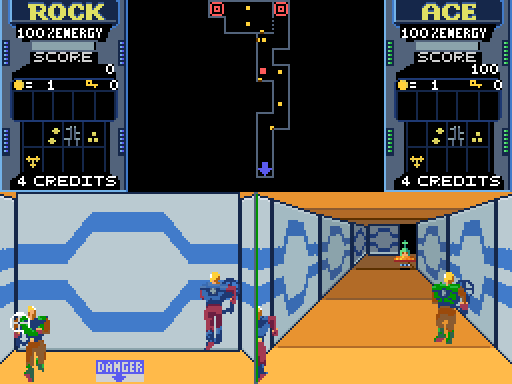
\includegraphics[width=0.48\textwidth]{../img/play_l1.png}\hfill
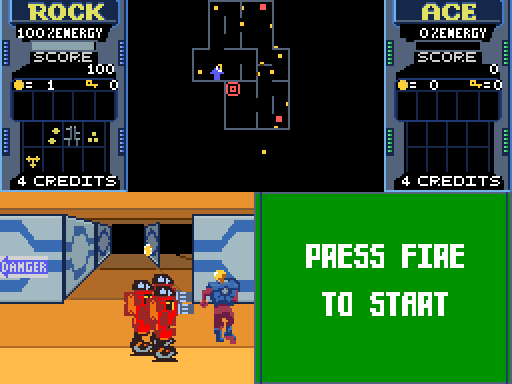
\includegraphics[width=0.48\textwidth]{../img/play_l5.png}
\caption{Izquierda: Rock y Ace en el primer nivel, cada uno en su vista. Derecha: robots en el nivel 5.}
\end{figure}

Rock (jugador 1) y Ace (jugador 2) recorren los laberintos de la ciudad de los Xybots, vistos desde detrás del héroe. Cada nivel es un
laberinto lleno de robots, monedas, llaves y energía. \textbf{Encuentra la salida del nivel y entra en ella.} Antes de empezar se muestra
el número del nivel (\texttt{PREPARE TO ENTER LEVEL}).

\begin{itemize}
\item \textbf{Robots.} Dispárales; los más duros necesitan varios impactos. Algunos se lanzan contra ti: el choque quita 25 de energía.
Los robots pueden recoger objetos y los sueltan al ser destruidos. También se pueden derribar algunas paredes a tiros.
\item \textbf{Energía.} Empiezas con 100. Baja despacio con el tiempo, y con cada disparo o choque que te alcanza. Al llegar a 0 el
héroe muere y se gasta un crédito (sección 8).
\item \textbf{Las llaves} abren las puertas marcadas en el mapa. Al entrar en una puerta cerrada se gasta una llave y la puerta desaparece.
\item \textbf{Las monedas} son el dinero de la tienda entre niveles (sección 7).
\item \textbf{Dos jugadores.} El jugador 2 puede unirse con la partida en marcha pulsando disparo; la vista de Ace dice
\texttt{PRESS FIRE TO START}. No se puede durante las pantallas de tienda, bonus y espera ni en una pelea con el Master Xybot. Desde el
nivel 6, \texttt{SHOTS HURT OTHER PLAYERS}: cuidado con no dar a tu compañero. Cuando un jugador muere, su compañero se queda con sus llaves.
\item \textbf{Tras la salida} vienen una pantalla de bonus (si la hay), la tienda y la pantalla \texttt{PREPARE}. En una partida de dos
jugadores, el primero en salir ve \texttt{WAITING...} hasta que llega su compañero, y recibe \texttt{BONUS FOR EXITING FIRST}: una moneda.
\item \textbf{Puntos}: cada objeto recogido da 100 puntos, y cada robot destruido también da puntos.
\end{itemize}

\begin{figure}[H]
\centering
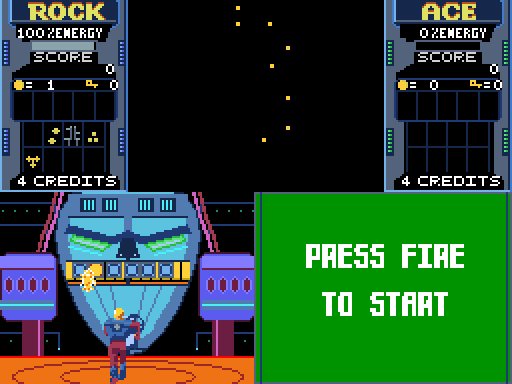
\includegraphics[width=0.48\textwidth]{../img/boss.png}\hfill
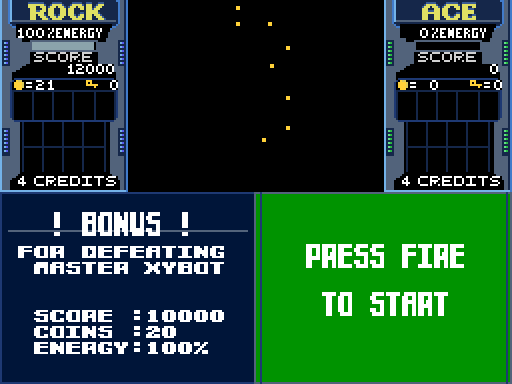
\includegraphics[width=0.48\textwidth]{../img/bonus_boss.png}
\caption{Izquierda: el Master Xybot. Derecha: el bonus por derrotarlo.}
\end{figure}

\textbf{El Master Xybot.} En lugar de los niveles 16, 26 y 36 te enfrentas al Master Xybot en su sala (\texttt{PREPARE TO FIGHT MASTER XYBOT};
la pantalla \texttt{PREPARE} te avisa unos niveles antes). Sus seis piezas se abren y se cierran, y disparan cuando están abiertas; solo
se les puede herir abiertas. Destruye las seis: \texttt{! BONUS !} da 10.000 puntos, 20 monedas y la energía completa, y la partida sigue
con el nivel siguiente. Si todos los jugadores mueren en la pelea, la partida retrocede cuatro niveles. Tras el último nivel el juego
vuelve a empezar desde el nivel 1, con robots más duros.

% ==================================================================
\sect{6. El panel}

Cada jugador tiene un panel: Rock a la izquierda y Ace a la derecha. El mapa está en el centro.

\begin{center}
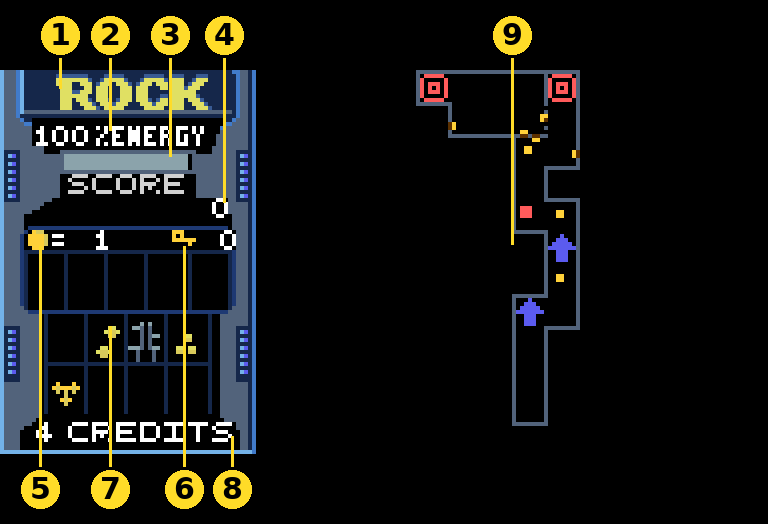
\includegraphics[width=0.85\textwidth]{img/hud.png}
\end{center}

\begin{tabularx}{\textwidth}{@{}clX@{}}
\toprule
\textbf{\tNo} & \textbf{\tElement} & \textbf{\tTellsYou}\\
\midrule
1 & Nombre & \texttt{ROCK} es el jugador 1 y \texttt{ACE} el jugador 2.\\
2 & \texttt{\char37{}ENERGY} & La energía que queda, de 0 a 100 (125 con \texttt{125\char37{} LIMIT}).\\
3 & Barra de energía & La misma energía en forma de barra.\\
4 & \texttt{SCORE} & Los puntos del jugador.\\
5 & Monedas & Las monedas que lleva el jugador, para gastar en la tienda.\\
6 & Llaves & Las llaves que lleva el jugador.\\
7 & Equipo & Un icono por cada mejora o accesorio de la tienda que tiene el jugador.\\
8 & \texttt{CREDITS} & Los créditos que quedan; los comparten los dos jugadores.\\
9 & Mapa & La parte del laberinto vista hasta ahora: paredes, puertas cerradas (de puntos), las salidas (un cuadrado dentro de otro), los
héroes (flechas que indican hacia dónde miran) y marcas de robots y objetos. En la sala del Master Xybot se queda vacío.\\
\bottomrule
\end{tabularx}

% ==================================================================
\sect{7. Objetos y la tienda}

\textbf{En el suelo:} monedas (una moneda), llaves (una llave), energía (50 o 100 de energía, nunca por encima del límite) y la mejora del
arma: durante un rato los disparos son más fuertes y el héroe dispara dos bolas a la vez, o tres si vuelve a cogerla.

\begin{figure}[H]
\centering
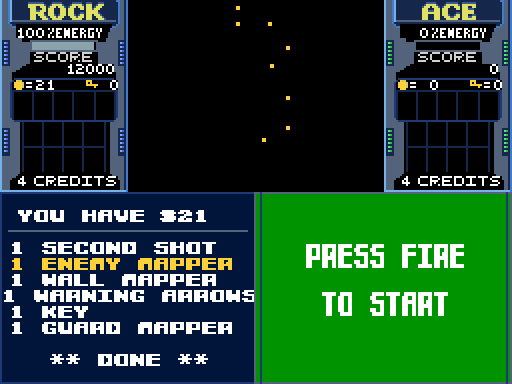
\includegraphics[width=0.55\textwidth]{../img/shop.png}
\caption{La tienda: \texttt{YOU HAVE \$21} monedas; arriba y abajo eligen y el disparo compra.}
\end{figure}

\textbf{La tienda} se abre tras cada salida si tienes monedas. Ofrece hasta seis cosas, con su precio en monedas delante. Arriba y
abajo mueven la barra y el disparo compra; \texttt{** DONE **} sale. La tienda se cierra sola cuando te quedas sin monedas. Las mejoras
se pueden comprar varias veces, hasta su máximo.

\begin{tabularx}{\textwidth}{@{}lcX@{}}
\toprule
\textbf{Artículo} & \textbf{Monedas} & \textbf{Qué hace}\\
\midrule
\texttt{MOVE FASTER} & 7 & Andas más rápido.\\
\texttt{BETTER SHIELD} & 7 & Los disparos hacen menos daño.\\
\texttt{FAST SHOTS} & 7 & Tus disparos vuelan más rápido.\\
\texttt{SHOT POWER} & 7 & Tus disparos hacen más daño.\\
\texttt{ZAP POWER} & 7 & Un ataque especial más fuerte (también gasta más energía).\\
\texttt{SLOW ENERGY} & 2 & La energía baja más despacio con el tiempo.\\
\texttt{SECOND SHOT} & 1 & Dos disparos en el aire a la vez.\\
\texttt{ENEMY MAPPER} & 1 & Los robots aparecen en el mapa.\\
\texttt{WALL MAPPER} & 1 & Todo el laberinto aparece en el mapa.\\
\texttt{GUARD MAPPER} & 1 & Los robots guardianes aparecen en el mapa.\\
\texttt{WARNING ARROWS} & 1 & Carteles \texttt{DANGER} a los lados de la vista cuando un robot puede llegar hasta ti en línea recta.\\
\texttt{50\char37{} ENERGY POD} & 5 & 50 de energía.\\
\texttt{SHOTS REPELLED} & 5 & Los cinco próximos disparos que te alcancen rebotan.\\
\texttt{125\char37{} LIMIT} & 5 & La energía puede subir hasta 125.\\
\texttt{KEY} & 1 & Una llave.\\
\texttt{GIVE FRIEND} & 1 & Da una moneda a tu compañero.\\
\bottomrule
\end{tabularx}

\medskip
Desde el nivel 7, los accesorios (segundo disparo, mapas, flechas de aviso, límite del 125\%) se gastan: cada salida les quita un nivel.

% ==================================================================
\sect{8. Créditos, continuar y récord}

\begin{itemize}
\item La partida empieza con \textbf{4 créditos}, compartidos por los dos jugadores (\texttt{4 CREDITS} en el panel).
\item Cuando un héroe muere, se gasta un crédito y la vista dice \texttt{PRESS FIRE TO CONTINUE}. El disparo devuelve al héroe al
principio del nivel con la energía completa y conservando todo lo comprado.
\item La muerte que gasta el \textbf{último crédito} termina la partida de ese jugador: si la puntuación supera el récord, parpadea
\texttt{NEW HISCORE}; después, \texttt{GAME OVER}. Con 4 créditos un jugador puede continuar tres veces.
\item El récord empieza en 1000 y se ve en la pantalla de título como \texttt{HI:}. Se conserva hasta que se apaga el MSX.
\item Unirse como jugador 2 no gasta créditos.
\end{itemize}

% ==================================================================
\sect{9. Música y voces}

Sin un Moonsound oyes la música y los efectos de sonido del juego original de MSX. Con un \textbf{Moonsound}, la música y las voces son:

\begin{itemize}
\item una canción con voces en la pantalla del logo;
\item la música de título de la recreativa, con sus voces, en la pantalla de título;
\item una de cuatro voces de la recreativa, al azar, al empezar la partida;
\item dos canciones de la recreativa en los niveles, una para los impares y otra para los pares;
\item la música de la tienda de la recreativa en la tienda y en la pantalla \texttt{PREPARE};
\item la música del Master Xybot y su voz: al empezar la pelea, cuando recibe un impacto y ``I'll be back'' cuando es derrotado.
\end{itemize}

Con más de 128~KB de RAM de muestras en el Moonsound, los disparos, los impactos y algunas recogidas, salidas y teletransportes usan sonidos de la recreativa. Los demás efectos siguen saliendo del MSX.

% ==================================================================
\sect{10. Consejos}

\begin{itemize}
\item Mira el mapa: las salidas se dibujan como un cuadrado dentro de otro. Las puertas necesitan llaves, así que recógelas por el camino.
\item Algunos niveles esconden una \textbf{salida de salto}: \texttt{WARP BONUS} te lleva directamente al nivel 7 con 25 monedas, la energía completa y 75.000 puntos.
\item Guarda monedas para la tienda: \texttt{SHOT POWER}, \texttt{BETTER SHIELD} y \texttt{SLOW ENERGY} ayudan a la larga.
\item El ataque especial limpia un pasillo lleno, pero gasta energía: úsalo cuando haya muchos robots a la vista.
\item En partidas de dos jugadores, salir el primero da una moneda; desde el nivel 6, no te pongas en la línea de tiro de tu compañero.
\item \key{P} pausa el juego en cualquier momento.
\end{itemize}
